\chapter{Dataset Construction}\label{chap:dataset-construction}
\section{Design Goals}

Our goal is to construct synthetic structured attributes that are going to be later used in our experiments. We generate two types of attributes: (i) correlated attributes, which are explicitly coupled to the geometry of the vector space, and (ii) uncorrelated attributes, which serve as a random baseline.

All attributes are defined over a bounded discrete domain:
\[
\mathcal{A} = \{0, 1, \dots, 200\}.
\]

\paragraph{Uncorrelated Attributes}

In contrast, uncorrelated attributes are generated independently of the vector space. Each vector is assigned a value uniformly at random from $\mathcal{A}$. This removes any relationship between vector similarity and attribute similarity and serves as a baseline to evaluate the effect of correlation.

\section{Correlated Attribute Generation}

We aim to enforce a strong relationship between vector similarity and attribute similarity, i.e., vectors that are close in the embedding space should receive similar attribute values.

To achieve this, we construct attributes that vary smoothly over the vector space. We first group similar vectors into clusters and assign each cluster a scalar value, which is then smoothly interpolated to all vectors. 

This results in attribute values that are consistent within local regions and change gradually across the space, without sharp cluster boundaries.

\subsection{Clustering}

Let $\{x_i\}_{i=1}^N \subset \mathbb{R}^d$ denote the set of base vectors.

To capture the geometric structure of the vector space, we first partition the dataset using clustering. Specifically, we apply MiniBatch $k$-means to obtain $k$ cluster centroids:
\[
\{c_j\}_{j=1}^k.
\]

These centroids serve as representative points that summarize the global distribution of the data.

\subsection{Cluster Anchors}
To induce a structured signal over the clusters, we assign each centroid a scalar anchor value.
Rather than relying on the arbitrary ordering induced by $k$-means, we first order the centroids
according to their projection onto the first principal component (PC1).

Let $\pi$ denote the permutation that sorts centroids along PC1. We then define:
\[
v_j = \frac{j-1}{k-1}, \quad j \in \{1, \dots, k\},
\]
where $c_j$ follows this ordering.

This ensures that nearby centroids in the embedding space receive similar anchor values,
preserving global geometric consistency.

\subsection{Gaussian Weighting}

For each vector $x_i$, we compute its squared Euclidean distance to all centroids:
\[
d_{ij} = \|x_i - c_j\|^2.
\]

We then define soft assignment weights using a Gaussian kernel:
\[
w_{ij} = \exp\left(-\frac{d_{ij}}{2\sigma^2}\right).
\]

\paragraph{Bandwidth Parameter}

The parameter $\sigma > 0$ is referred to as the \emph{bandwidth} of the kernel. It controls how quickly the influence of a centroid decays as a function of distance.

\begin{itemize}
    \item If $\sigma$ is small, only very close centroids receive significant weight, resulting in highly localized assignments.
    \item If $\sigma$ is large, many centroids contribute similarly, leading to smoother but less discriminative assignments.
\end{itemize}

Thus, $\sigma$ determines the scale at which the geometry of the space is observed and directly influences the strength of the induced correlation between vectors and attributes.

\paragraph{Bandwidth Estimation}

A naive computation of $\sigma$ based on all pairwise distances $\|x_i - c_j\|$ would require $\mathcal{O}(|S|k)$ operations, which is computationally expensive for large-scale datasets.

To address this, we estimate $\sigma$ using a random subsample. Let $S \subset \{1,\dots,N\}$ be a uniformly sampled subset with $|S| = \min(10^4, N)$. We define:
\[
\sigma = \operatorname{median}\left(\{ \|x_i - c_j\| : i \in S, \; j \in \{1,\dots,k\} \}\right).
\]

\paragraph{Why the Median?}

We use the median of the sampled distances to estimate $\sigma$ instead of the mean in order to obtain a robust estimate of the characteristic distance scale.

In high-dimensional spaces, distance distributions often exhibit heavy tails and may contain outliers (e.g., points far from any centroid). The mean is sensitive to such extreme values and can be significantly skewed, leading to an overestimation of $\sigma$. This, in turn, would cause the Gaussian kernel to become overly flat, reducing locality and weakening the correlation between geometry and the generated attribute.

In contrast, the median is a robust statistic that is insensitive to outliers and better reflects the typical (central) distance between vectors and centroids. As a result, it yields a more stable and representative bandwidth, ensuring that the kernel maintains an appropriate balance between locality and smoothness.

\paragraph{Monte Carlo Interpretation}

This estimation can be viewed as a Monte Carlo approximation of the global distance distribution between data points and centroids.

Specifically, instead of computing statistics over the full set of $Nk$ distances, we approximate the median distance by sampling a subset of points uniformly at random. Under this sampling scheme, the empirical distribution of distances over $S$ converges to the true distribution as $|S|$ increases. Therefore, the estimated $\sigma$ provides a consistent approximation of the characteristic distance scale of the dataset, while significantly reducing computational cost.

\subsection{Soft Assignment}

The weights $w_{ij}$ induce a \emph{soft assignment} of each vector to all clusters simultaneously.

In contrast to hard clustering, where each vector is assigned to a single cluster:
\[
x_i \mapsto \arg\min_j \|x_i - c_j\|,
\]
soft assignment produces a distribution over clusters:
\[
x_i \mapsto (w_{i1}, w_{i2}, \dots, w_{ik}).
\]

Each weight $w_{ij}$ reflects the degree to which centroid $c_j$ contributes to the representation of $x_i$. Nearby centroids receive higher weights, while distant centroids contribute negligibly.

This has two key advantages:
\begin{itemize}
    \item It avoids discontinuities introduced by hard assignments, where small changes in $x_i$ may abruptly change cluster membership.
    \item It allows multiple nearby clusters to jointly influence the attribute value, leading to smoother and more robust metadata.
\end{itemize}

\subsection{Radial Basis Function Interpretation}

The Gaussian kernel used in the weighting scheme is a specific instance of a \emph{radial basis function} (RBF). In general, an RBF is a function of the form:
\[
\phi(x, c) = g(\|x - c\|),
\]
i.e., its value depends only on the distance between $x$ and a center $c$.

In our case:
\[
\phi(x_i, c_j) = \exp\left(-\frac{\|x_i - c_j\|^2}{2\sigma^2}\right).
\]

The term ``radial'' refers to the fact that the function is isotropic—it depends only on the radius (distance) and not on direction.

\paragraph{Why RBFs are used}

Using an RBF provides the following properties:

\begin{itemize}
    \item \textbf{Smooth decay:} The influence of a centroid decreases smoothly with distance, avoiding sharp boundaries.
    
    \item \textbf{Locality:} Only nearby centroids contribute significantly, preserving local geometric structure.
    
    \item \textbf{Continuity:} The resulting mapping from vectors to attributes is continuous, ensuring that similar vectors receive similar attribute values.
\end{itemize}

These properties are essential for constructing metadata that is meaningfully correlated with the geometry of the embedding space. In particular, the RBF weighting ensures that the resulting attributes respect the underlying notion of similarity induced by the vector representation.

\subsection{Continuous Attribute Construction}

We define the continuous attribute value for each vector as:
\[
a_i^{(\mathrm{cont})} =
\frac{\sum_{j=1}^k w_{ij} v_j}{\sum_{j=1}^k w_{ij}}.
\]

This corresponds to a kernel-weighted aggregation of cluster-level signals.

\paragraph{Marginal Flattening}

To reduce skew in the attribute distribution, we apply a rank-based rescaling to $a_i^{(\mathrm{cont})}$.

Specifically, we replace each value by its empirical cumulative distribution function (CDF) rank:
\[
a_i^{(\mathrm{cont})} \leftarrow \frac{\mathrm{rank}(a_i^{(\mathrm{cont})})}{N}.
\]

This transformation preserves ordering while producing a more uniform marginal distribution, improving the stability of neighbor comparisons.

\paragraph{Normalization and Quantization}

We normalize:
\[
\hat{a}_i = \frac{a_i^{(\mathrm{cont})} - \min_i a_i^{(\mathrm{cont})}}
{\max_i a_i^{(\mathrm{cont})} - \min_i a_i^{(\mathrm{cont})}},
\]
with appropriate handling for degenerate cases.

Finally, we quantize:
\[
a_i = \mathrm{round}(200 \cdot \hat{a}_i), \quad a_i \in \{0,\dots,200\}.
\]

This yields discrete attributes suitable for range-based filtering.

\begin{figure}[t]
    \centering
    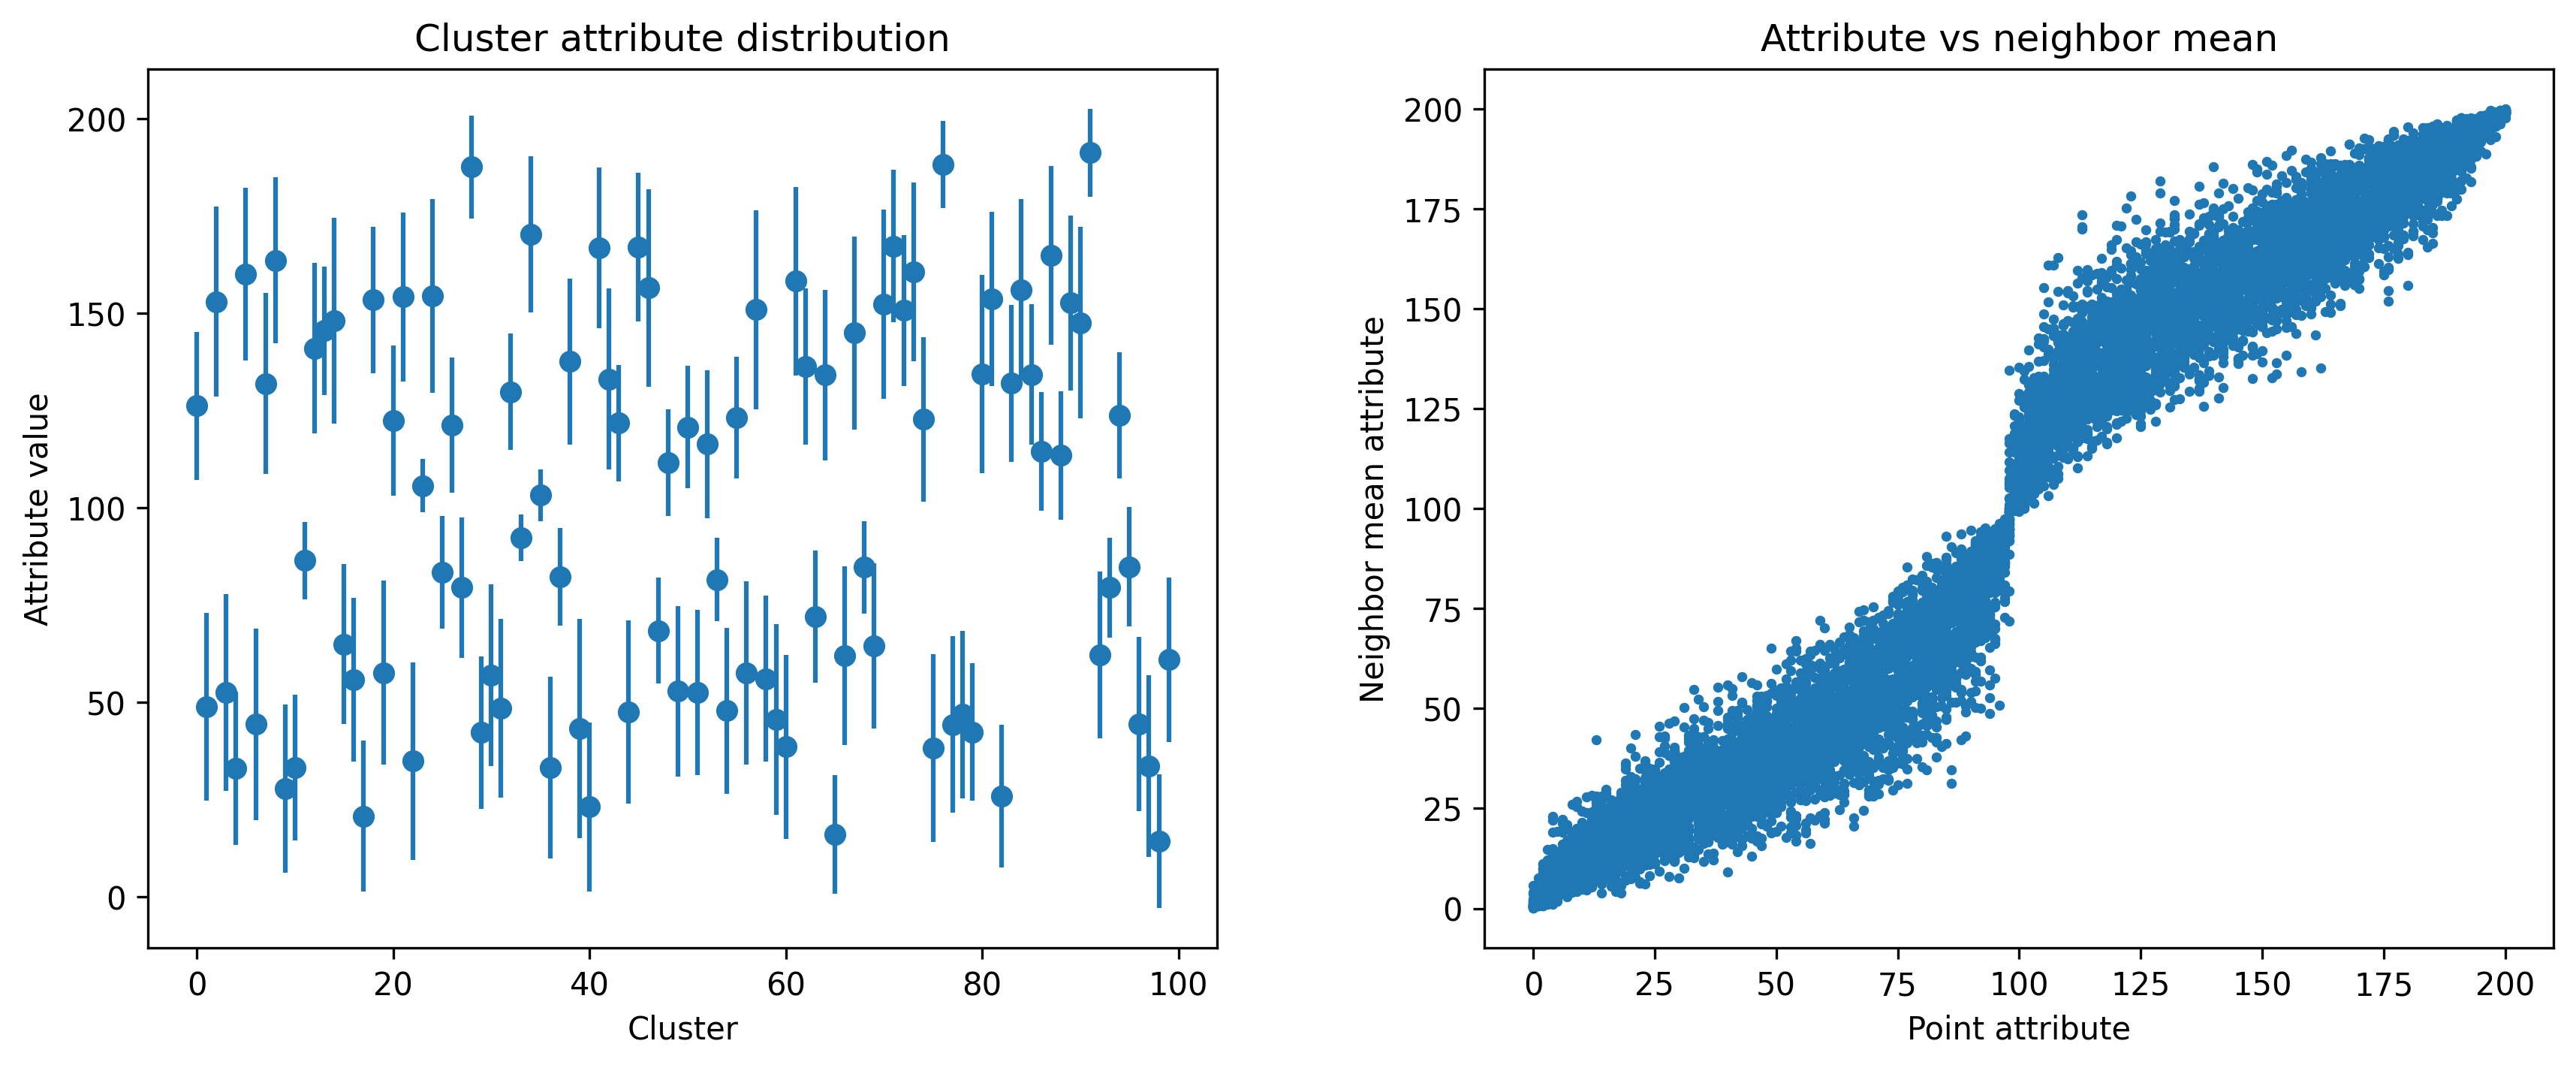
\includegraphics[width=0.8\linewidth]{figures/correlated_attr_stats.png}
    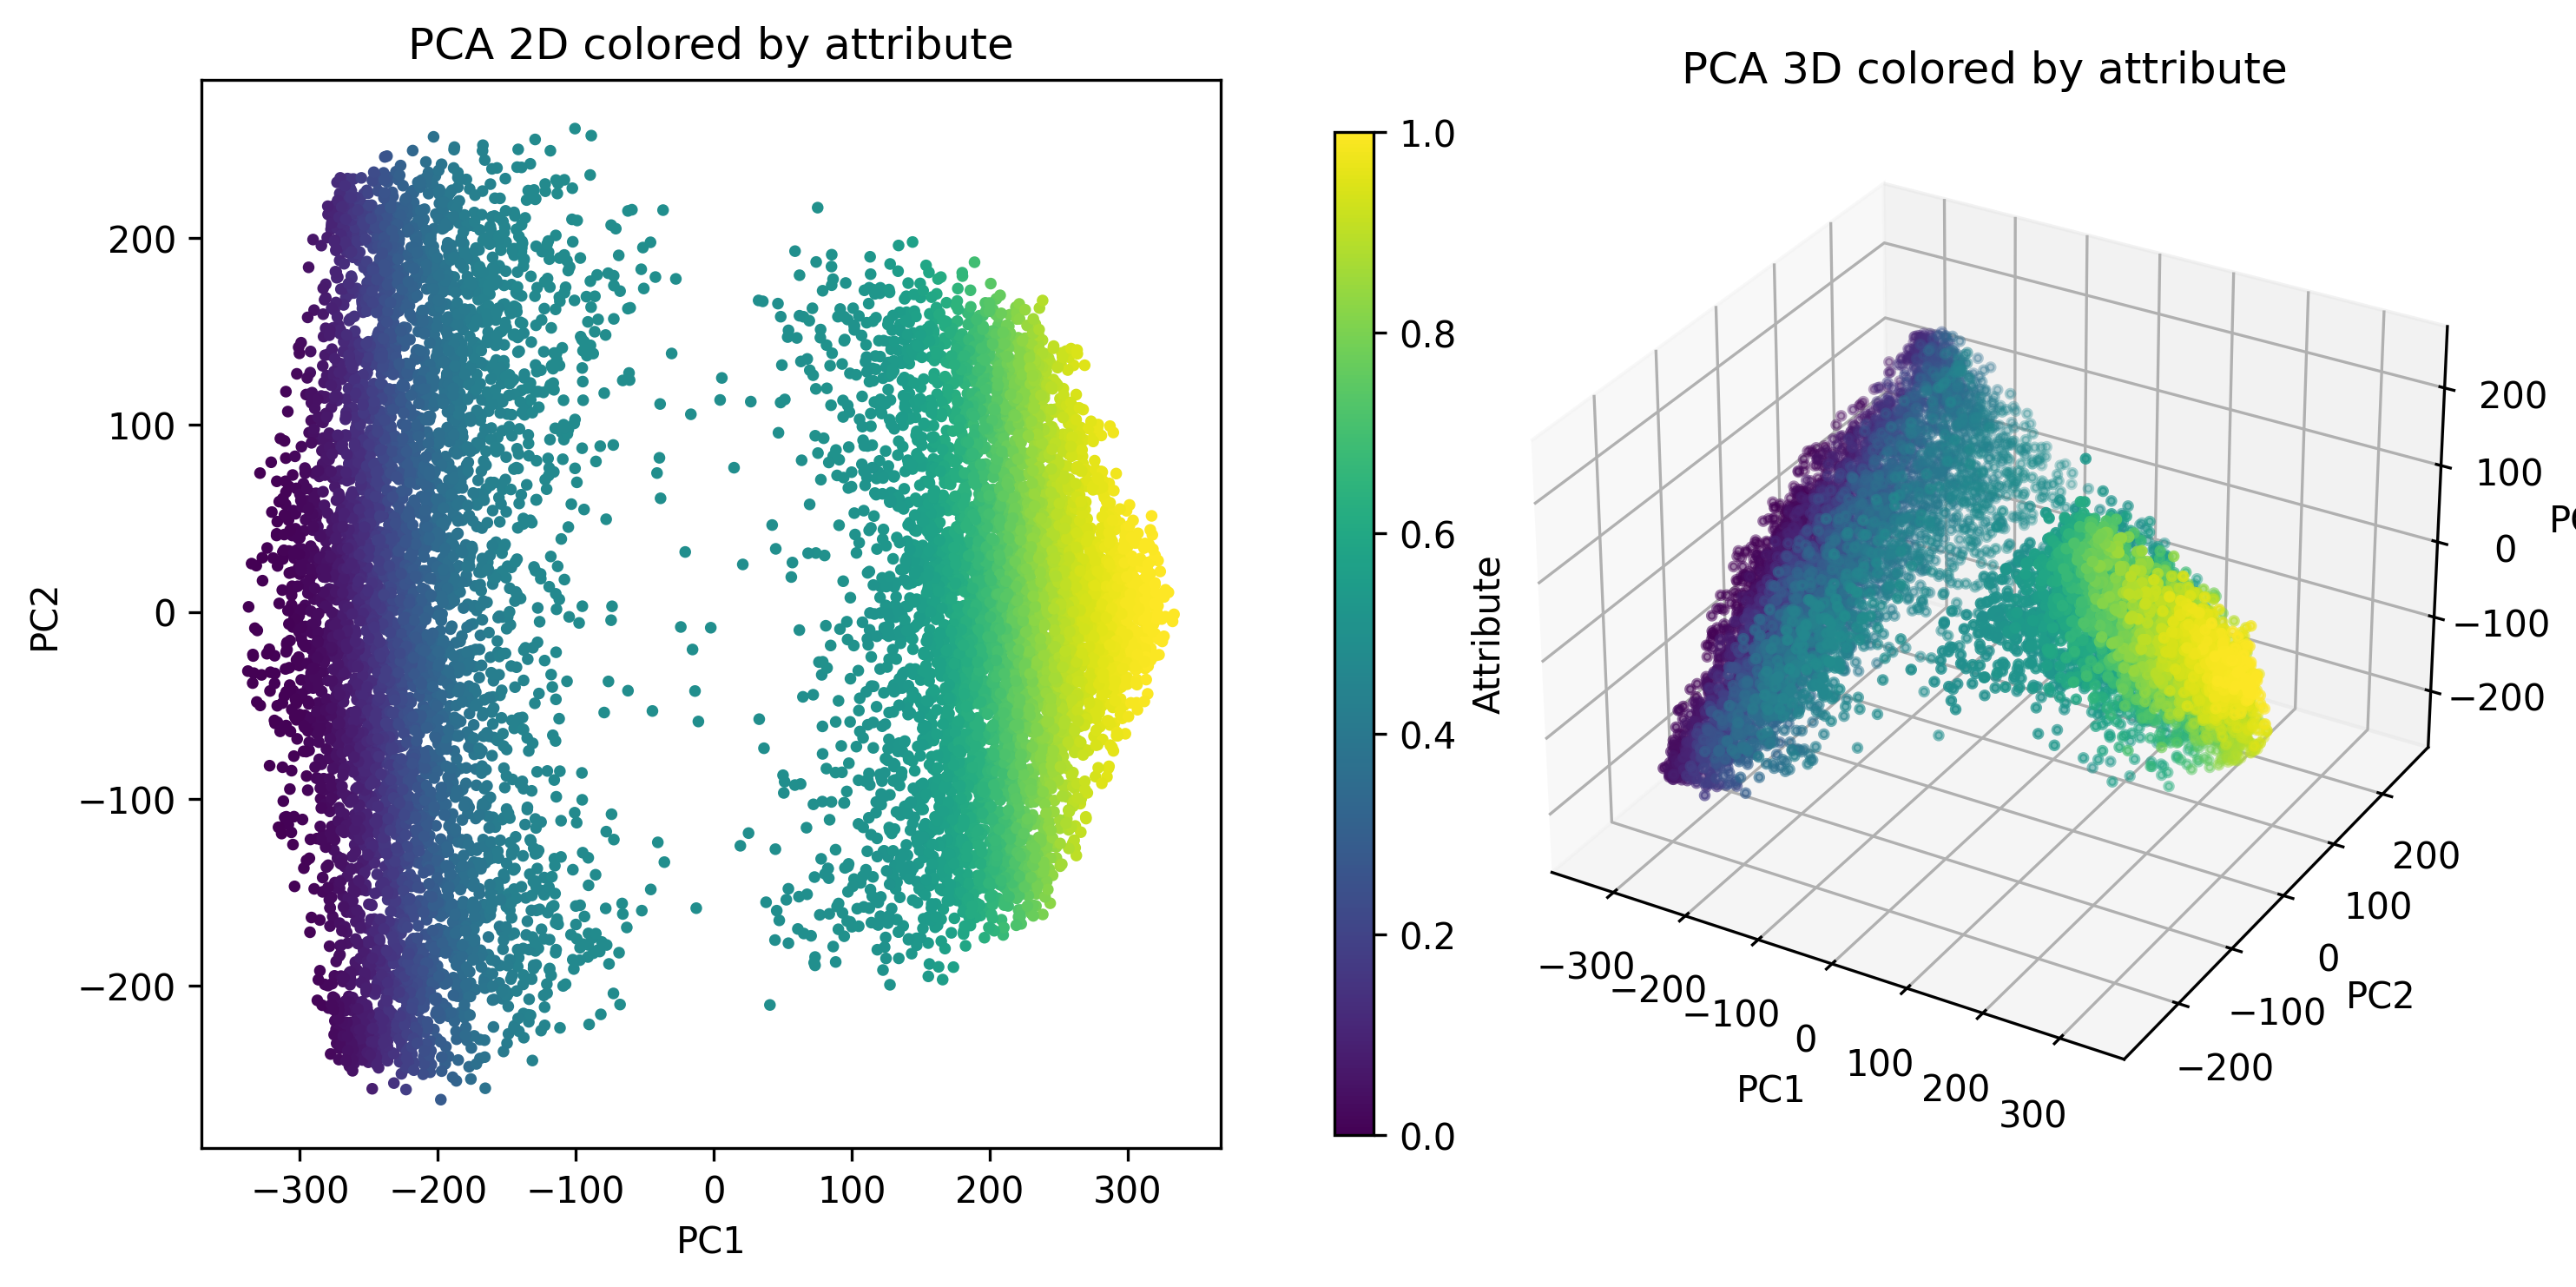
\includegraphics[width=0.8\linewidth]{figures/correlated_attr_pca_pair.png}
    \caption{Your caption describing the image.}
    \label{fig:your_label}
\end{figure}

\section{Uncorrelated Attribute Generation}

\section{Query Range Generation}
\subsection{Positive (correlated)}
\subsection{Negative (anti-correlated)}
\subsection{Random}

\section{Selectivity Control}

\section{Dataset Validation}
\subsection{Neighbor consistency}
\subsection{Cluster distributions}
